\subsection{Nonabelian Examples}


%%%%%%%%%%%%%%%%%%%%%%%%%%%%%%
%  Notation and Terminology  %
%%%%%%%%%%%%%%%%%%%%%%%%%%%%%%

\subsubsection{Notation and Terminology}

Algebraists usually do not use the symbol $*$ to denote the group operation. Instead, they often use juxtaposition, so that $a*b$ is denoted by $ab$. In this case, the identity element is denoted by $1$ or $e$, and the inverse of an element $a$ is denoted by $a^{-1}$ instead of $a'$. When we write $ab$, we mean the product of $a$ and $b$ under the group operation. The notation $a+b$ is also often used to denote the group operation, especially when the group is Abelian. When the group operation is denoted by $+$, the identity element is denoted by $0$, and the inverse of an element $a$ is denoted by $-a$. When we write $a+b$, we mean the sum of $a$ and $b$ under the group operation.

\Note[Summary]{
    \begin{center}
        \begin{tabular}{c|c|c}
            $\cdot$ Notation & $+$ Notation \\ \hline
            May or may not be Abelian & Abelian \\
            \hline
            $e$ & $0$ \\
            $a^{-1}$ & $-a$ \\
            $ab$ & $a+b$ \\
            $a^k$ & $ka$ \\
            $a^{-k}$ & $-ka$ \\
            $a^0 = 1$ & $0a = 0$ \\
            $a^{n+m} = a^n a^m$ & $(n+m)a = na + ma$ \\
            $(a^n)^m = a^{nm}$ & $m(na) = (mn)a$ \\
            \hline
        \end{tabular}
    \end{center}
}

\Definition{Order of group}{
    The \textbf{order} of a group $G$, denoted by $|G|$, is the number of elements in $G$.
}


%%%%%%%%%%%%%%%%%%%%%%%%
%  Permutation Groups  %
%%%%%%%%%%%%%%%%%%%%%%%%

\subsubsection{Permutation Groups}

\Definition{Permutation}{
    A \textbf{permutation} of a set $A$ is a bijection $\sigma : A \to A$.
}

\Definition{Permutation multiplication}{
    Function composition $\circ$ is a binary operation on the collection of all permutations of a set $A$. We call this operation \textbf{permutation multiplication}.

    Let $\sigma$ and $\tau$ be permutations of $A$. The composite function $\sigma \circ \tau$ defined schematically by \[ 
        A \xrightarrow{\tau} A \xrightarrow{\sigma} A
    \]
    gives a bijection from $A$ to $A$, and hence is a permutation of $A$.
}

\Lemma{}{
    The permutation multiplication is bijective.
}

\Proof{
    Let $\sigma$ and $\tau$ be permutations of $A$. Let's first show that $\sigma\tau$ is injective. If $(\sigma\tau)(a_1) = (\sigma\tau)(a_2)$, then $\sigma(\tau(a_1)) = \sigma(\tau(a_2))$. Since $\sigma$ is injective, we have $\tau(a_1) = \tau(a_2)$. And since $\tau$ is injective, we conclude that $a_1 = a_2$, so $\sigma\tau$ is injective.

    To show that $\sigma\tau$ is surjective, let $b \in A$. Since $\sigma$ is surjective, there exists $a \in A$ such that $\sigma(a) = b$. Since $\tau$ is surjective, there exists $c \in A$ such that $\tau(c) = a$. Thus, we have $(\sigma\tau)(c) = \sigma(\tau(c)) = \sigma(a) = b$, so $\sigma\tau$ is surjective. Hence, $\sigma\tau$ is bijective.
}

\Example{}{
    Suppose that \[ 
        A = \{ 1,2,3,4,5 \}
    \]
    and that $\sigma$ is the permutation given by the following diagram: \[ 
        \begin{matrix}
            1 & 2 & 3 & 4 & 5 \\
            \downarrow & \downarrow & \downarrow & \downarrow & \downarrow \\
            4 & 2 & 5 & 3 & 1
        \end{matrix}
    \]
    and $\tau$ is the permutation given by the following diagram: \[ 
        \begin{matrix}
            1 & 2 & 3 & 4 & 5 \\
            \downarrow & \downarrow & \downarrow & \downarrow & \downarrow \\
            3 & 5 & 4 & 2 & 1
        \end{matrix}
    \]
    Then we can write $\sigma$ and $\tau$ in two-row notation as
    \begin{align*}
        \sigma &= \begin{pmatrix} 1 & 2 & 3 & 4 & 5 \\ 4 & 2 & 5 & 3 & 1 \end{pmatrix} \\
        \tau &= \begin{pmatrix} 1 & 2 & 3 & 4 & 5 \\ 3 & 5 & 4 & 2 & 1 \end{pmatrix}
    \end{align*}
    Then the convolution can be written as:
    \begin{align*}
        \sigma\tau &= \begin{pmatrix} 1 & 2 & 3 & 4 & 5 \\ 4 & 2 & 5 & 3 & 1 \end{pmatrix} \begin{pmatrix} 1 & 2 & 3 & 4 & 5 \\ 3 & 5 & 4 & 2 & 1 \end{pmatrix} \\
                   &= \begin{pmatrix} 1 & 2 & 3 & 4 & 5 \\ \sigma(3) & \sigma(5) & \sigma(4) & \sigma(2) & \sigma(1) \end{pmatrix} \\
                   &= \begin{pmatrix} 1 & 2 & 3 & 4 & 5 \\ 5 & 1 & 3 & 2 & 4 \end{pmatrix}
    \end{align*}
}

\Theorem{}{
    Let $A$ be a nonempty set, and let $S_A$ be the collection of all permutations of $A$. Then $S_A$ is a group under permutation multiplication.
}

\Proof{
    We first check that $S_A$ is closed under permutation multiplication. Let $\sigma$ and $\tau$ be permutations of $A$. Then $\sigma\tau$ is a permutation of $A$, so $\sigma\tau \in S_A$.

    Since function composition is associative, we have that permutation multiplication is associative, which verifies $\G_1$.

    The permutation $\iota$ such that $\iota(a) = a$ for all $a \in A$acts as identity. Therefore, $\G_2$ is satisfied.

    For a permutation $\sigma$, the inverse function $\sigma^{-1}$ is the permutation that reverses the direction of the mapping $\sigma$.

    The existence of exactly one such element $\sigma^{-1}$ is guaranteed by the fact that $\sigma$ is a bijection. Thus, $\G_3$ is satisfied, and $S_A$ is a group under permutation multiplication.
}

\Definition{Symmetric Group}{
    Let $A$ be the finite set $\{1, 2, \ldots, n\}$. The group of all permutations of $A$ is the \textbf{symmetric group on $n$ letters}, and is denoted by $S_n$.
}

\Note{
    $S_n$ has $n!$ elements, where $n! = n(n-1)(n-2)\cdots(3)(2)(1)$.
}

\Example{}{
    Let $\sigma = \begin{pmatrix} 1 & 2 & 3 \\ 2 & 1 & 3 \end{pmatrix}$ and $\tau = \begin{pmatrix} 1 & 2 & 3 \\ 1 & 3 & 2 \end{pmatrix}$. Then $\sigma\tau(1) = \sigma(1) = 2$, but $\tau\sigma(1) = \tau(2) = 3$. Thus $\sigma\tau \neq \tau\sigma$, so $S_3$ is not Abelian. We have seen that any group with at most four elements is Abelian. Furthermore, up to isomorphism, the Abelian group $\Z_5$ is the only group of order 5. Thus $S_3$ is the smallest group which is not Abelian.
}


%%%%%%%%%%%%%%%%%%%%%
%  Disjoint Cycles  %
%%%%%%%%%%%%%%%%%%%%%

\subsubsection{Disjoint Cycles}

There is a more efficient way of specifying the action of a permutation. In the two-row notation, we list each number 1 through $n$ twice. Disjoint cycle notation allows us to write the permutation using each number only once.

Let $\sigma = \begin{pmatrix} 1 & 2 & 3 & 4 & 5 & 6 \\ 3 & 4 & 6 & 2 & 5 & 1 \end{pmatrix}$. To write in disjoint cycle notation, we start by writing \[
    (1
\] We see that $\sigma(1) = 3$, so we write: \[
    (1, 3
\] Now $\sigma$ maps 3 to 6, so we write: \[
    (1, 3, 6
\] Our permutation maps 6 back to 1, so we place a parenthesis after 6: \[
    (1, 3, 6)
\]
This is called a \textbf{cycle} because when we apply $\sigma$ repeatedly, we cycle through the numbers 1, 3, and 6. A cycle containing exactly $k$ numbers is called a $k$-cycle. So $(1, 3, 6)$ is a 3-cycle.

We start another cycle for the remaining elements: $\sigma$ maps 2 to 4 and 4 maps back to 2, giving the 2-cycle \[
    (2, 4)
\] Since 5 maps to itself, we omit it. Thus in disjoint cycle notation, \[
    \sigma = (1, 3, 6)(2, 4)
\]

A 2-cycle is called a \textbf{transposition}. A collection of cycles is said to be \textbf{disjoint} if no entry is in more than one cycle. Disjoint cycles commute with each other.

\Example{}{
    In disjoint cycle notation, $\sigma \in S_9$ is written as $(1, 5, 2, 7)(3, 4, 9)$. Reading off the disjoint cycle notation, $\sigma(1) = 5, \sigma(5) = 2, \sigma(2) = 7, \sigma(7) = 1, \sigma(3) = 4, \sigma(4) = 9, \sigma(9) = 3$. Since 6 and 8 do not appear in either cycle, $\sigma(6) = 6$ and $\sigma(8) = 8$. Thus in two-row notation,
    \[
        \sigma = \begin{pmatrix}
            1 & 2 & 3 & 4 & 5 & 6 & 7 & 8 & 9 \\
            5 & 7 & 4 & 9 & 1 & 6 & 2 & 8 & 3
        \end{pmatrix}
    \]
}

\Lemma{}{
    Disjoint cycles commute with each other.
}

\Proof{
    Let $\sigma$ and $\tau$ be disjoint cycles. Let $a \in \{1, 2, \ldots, n\}$. If $a$ is not in either cycle, then $\sigma\tau(a) = a = \tau\sigma(a)$. If $a$ is in $\sigma$ but not in $\tau$, then $\tau(a) = a$, so $\sigma\tau(a) = \sigma(a)$ and $\tau\sigma(a) = \tau(\sigma(a)) = \sigma(a)$, so $\sigma\tau(a) = \tau\sigma(a)$. If $a$ is in $\tau$ but not in $\sigma$, then $\sigma(a) = a$, so $\sigma\tau(a) = \sigma(\tau(a)) = \tau(a)$ and $\tau\sigma(a) = \tau(a)$, so $\sigma\tau(a) = \tau\sigma(a)$. Thus, for all $a$, we have $\sigma\tau(a) = \tau\sigma(a)$, so $\sigma\tau = \tau\sigma$.
}

\Example{Let $\sigma=(1,5,3,2,6)$ and $\tau=(1,2,4,3,6)$ in $S_6$. Find $\sigma\tau$ in disjoint cycle notation without writing $\sigma$ and $\tau$ in two-row notation.}{
    \[ \sigma\tau = (1,5,3,2,6) (1,2,4,3,6) \]
    Since the operation is function composition, we see that the cycle $\tau$ on the right sends $1$ to $2$ and then the cycle on the left sends $2$ to $6$. So, $\sigma\tau(1)=6$ and so we can start writing \[ 
        \sigma\tau = (1,6
    \] Now we see that $\tau$ maps $6$ to $1$ and $\sigma$ maps $1$ to $5$. So, \[ 
        \sigma\tau = (1,6,5
    \] Next, $\tau(5) = 5$ and $\sigma(5) = 3$, so \[
        \sigma\tau = (1,6,5,3
    \] Next, $\tau(3) = 6$ and $\sigma(6) = 1$, so \[
        \sigma\tau = (1,6,5,3,1
    \] Since we have come back to $1$, we close the parenthesis: \[
        \sigma\tau = (1,6,5,3)
    \] Next, we look for the smallest number not in the cycle we just wrote. The smallest number not in the cycle is $2$. We have $\tau(2) = 4$ and $\sigma(4) = 4$, so we write \[
        \sigma\tau = (1,6,5,3)(2,4
    \] Next, $\tau(4) = 3$ and $\sigma(3) = 2$. Since we have come back to $2$, we close the parenthesis: \[
        \sigma\tau = (1,6,5,3)(2,4)
    \] Finally, we check if there are any numbers not in either cycle. The only number not in either cycle is $6$, but $6$ maps to itself, so we can omit it. 

    Thus, $\sigma\tau = (1,6,5,3)(2,4)$.
}

\Example{Compute the inverse of $\sigma = (1,5,7)(3,8,2,4,6)$}{
    In general, for a group $(ab)^{-1} = b^{-1}a^{-1}$, so \[ 
        \sigma^{-1} = (3,8,2,4,6)^{-1} (1,5,7)^{-1}
    \]
    The inverse of a cycle is simply written backward: \[ 
        \sigma^{-1} = (6,4,2,8,3)(7,5,1)
    \]
    However, since disjoint cycles commute, we can start each cycle with any entry in the cycle. So we could write \[
        \sigma^{-1} = (7,5,1)(6,4,2,8,3)
    \] or \[
        \sigma^{-1} = (1,7,5)(2,8,3,6,4)
    \]
}

\Note{
    The inverse of a cycle is simply the cycle written backward. For example, $(1, 5, 7)^{-1} = (7, 5, 1)$.
}

\Example{
    \begin{enumerate}[label=(\alph*)]
        \item Verify that the six matrices form a group under matrix multiplication.
            \[ 
                \mI,\ \mA,\ \mB,\ \mC,\ \mD,\ \mE
            \]
        \item What group discussed in this section is this group isomorphic to?
    \end{enumerate}
}{
    \begin{enumerate}[label=(\alph*)]
        \item
            We first check that the set of matrices is closed under matrix multiplication. Let $A$ and $B$ be any two of the six matrices. Then $AB$ is a matrix with exactly one entry of $1$ in each row and column, and all other entries are $0$. Thus, $AB$ is one of the six matrices, so the set of matrices is closed under matrix multiplication.

            Since matrix multiplication is associative, we have that matrix multiplication in this set is associative, which verifies $\G_1$.

            The identity matrix $\mI$ serves as the identity element, verifying $\G_2$.

            For each of the six matrices, we can find an inverse matrix in the set such that their product is the identity matrix. Thus, $\G_3$ is satisfied, and the set of matrices forms a group under matrix multiplication.
        \item This group is isomorphic to $S_3$, the symmetric group on three letters, since the six matrices correspond to the six permutations of three elements. For example, the matrix \[
            \mA
        \] corresponds to the permutation that sends $1$ to $2$, $2$ to $3$, and $3$ to $1$, which is the cycle $(1, 2, 3)$ in $S_3$. The other matrices correspond to the other permutations in $S_3$ in a similar way. Thus, the group of matrices is isomorphic to $S_3$.
    \end{enumerate}
}


%%%%%%%%%%%%%%%%%%%%%%%%
%  The Dihedral Group  %
%%%%%%%%%%%%%%%%%%%%%%%%

\subsubsection{The Dihedral Group}

To define the dihedral group, we first set up coordinates. Let $P_n$ denote the regular $n$-gon inscribed in the unit circle centered at the origin. We label the vertices with elements of $\Z_n$: vertex $k$ is placed at angle $\displaystyle \frac{2\pi k}{n}$ measured counterclockwise from the positive $x$-axis. So vertex $0$ sits at $(1, 0)$, vertex $1$ at $\displaystyle \left(\cos\frac{2\pi}{n}, \sin\frac{2\pi}{n}\right)$, and so on. The edges of $P_n$ are the line segments between vertices $k$ and $k +_n 1$ for $0 \leq k \leq n-1$.

\begin{figure}[H]
    \centering
    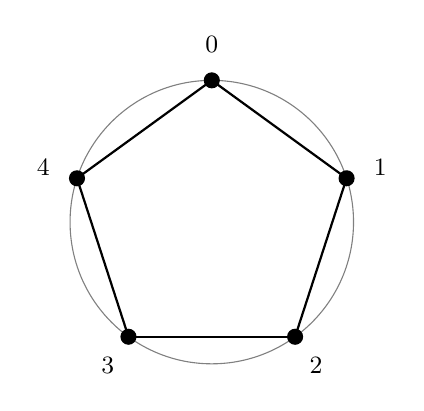
\begin{tikzpicture}[scale=1.8, every node/.style={font=\small}]
        \def\n{5}
        \draw[gray, thin] (0,0) circle (1);
    % Draw edges
        \foreach \k in {0,...,4} {
            \pgfmathtruncatemacro{\next}{mod(\k+1,\n)}
            \pgfmathsetmacro{\angA}{90 - \k * 360/\n}
            \pgfmathsetmacro{\angB}{90 - \next * 360/\n}
            \draw[thick] (\angA:1) -- (\angB:1);
        }
    % Draw vertices and labels
        \foreach \k in {0,...,4} {
            \pgfmathsetmacro{\ang}{90 - \k * 360/\n}
            \filldraw (\ang:1) circle (1.5pt);
            \node at (\ang:1.25) {$\k$};
        }
    \end{tikzpicture}
    \caption{The regular pentagon $P_5$ with vertex labels in $\Z_5$}
\end{figure}

\Definition{Dihedral Group}{
    The \textbf{dihedral group} $D_n$ is the set of all bijections $\phi : \Z_n \to \Z_n$ such that for any $i, j \in \Z_n$, the line between vertices $i$ and $j$ is an edge of $P_n$ if and only if the line between $\phi(i)$ and $\phi(j)$ is an edge of $P_n$.
}

\Note{
    In other words, the elements of $D_n$ are the symmetries of the regular $n$-gon: the bijections of the vertex set that preserve the edge structure.
}

\Theorem{}{
    For any $n \geq 3$, $\langle D_n,\circ \rangle$ is a group.
}

\Proof{
    Let $\phi, \theta \in D_n$ and suppose the line between vertices $i$ and $j$ is an edge of $P_n$. Since $\theta \in D_n$, the line between $\theta(i)$ and $\theta(j)$ is an edge. Since $\phi \in D_n$, the line between $\phi(\theta(i))$ and $\phi(\theta(j))$ is an edge. The converse direction follows similarly. Since the composition of bijections is a bijection, $\phi \circ \theta \in D_n$.

    Function composition is associative ($\G_1$). The identity function $\iota(k) = k$ preserves all edges ($\G_2$). For any $\phi \in D_n$, the inverse function $\phi^{-1}$ is also a bijection preserving edges ($\G_3$), since $\phi$ maps edges to edges if and only if $\phi^{-1}$ does.
}


%%% The generators rho and mu %%%

\subsubsection*{The generators $\rho$ and $\mu$}

Two fundamental elements of $D_n$ are \textbf{rotation} $\rho$ and \textbf{reflection} $\mu$:

\begin{itemize}
    \item $\rho : \Z_n \to \Z_n$ defined by $\rho(k) = k +_n 1$ (rotation by $2\pi/n$ counterclockwise). This sends each vertex to the next one around the circle.
    \item $\mu : \Z_n \to \Z_n$ defined by $\mu(k) = -k = n - k$ for $k > 0$ and $\mu(0) = 0$ (reflection across the $x$-axis, i.e., the line through vertex $0$ and the center).
\end{itemize}

\begin{figure}[H]
    \centering
    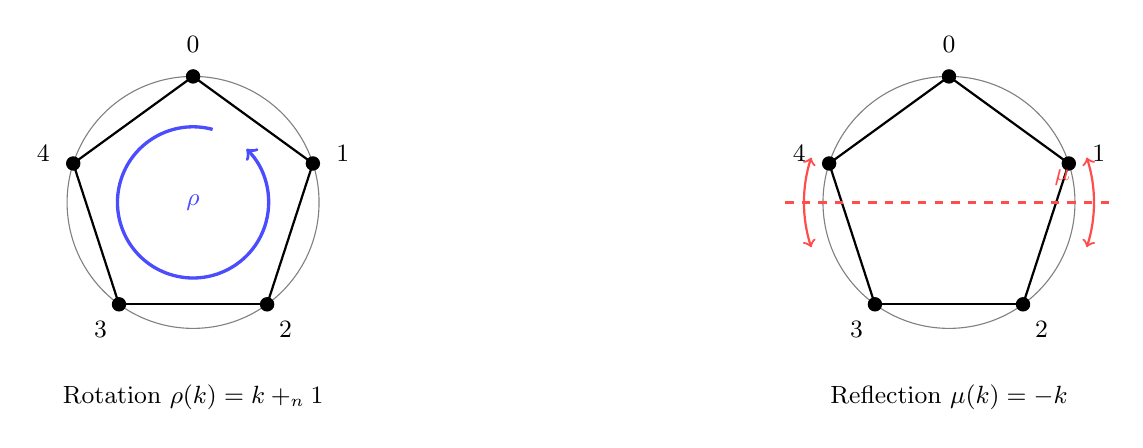
\begin{tikzpicture}[scale=1.6, every node/.style={font=\small}]
    % LEFT: Rotation
        \begin{scope}[xshift=-3cm]
            \def\n{5}
            \draw[gray, thin] (0,0) circle (1);
            \foreach \k in {0,...,4} {
                \pgfmathtruncatemacro{\next}{mod(\k+1,\n)}
                \pgfmathsetmacro{\angA}{90 - \k * 360/\n}
                \pgfmathsetmacro{\angB}{90 - \next * 360/\n}
                \draw[thick] (\angA:1) -- (\angB:1);
            }
            \foreach \k in {0,...,4} {
                \pgfmathsetmacro{\ang}{90 - \k * 360/\n}
                \filldraw (\ang:1) circle (1.5pt);
                \node at (\ang:1.25) {$\k$};
            }
        % Rotation arrow
            \draw[->, thick, blue!70, line width=1.2pt] (75:0.6) arc (75:405:0.6);
            \node[blue!70] at (0, 0) {$\rho$};
            \node at (0, -1.55) {Rotation $\rho(k) = k +_n 1$};
        \end{scope}

    % RIGHT: Reflection
        \begin{scope}[xshift=3cm]
            \def\n{5}
            \draw[gray, thin] (0,0) circle (1);
            \foreach \k in {0,...,4} {
                \pgfmathtruncatemacro{\next}{mod(\k+1,\n)}
                \pgfmathsetmacro{\angA}{90 - \k * 360/\n}
                \pgfmathsetmacro{\angB}{90 - \next * 360/\n}
                \draw[thick] (\angA:1) -- (\angB:1);
            }
            \foreach \k in {0,...,4} {
                \pgfmathsetmacro{\ang}{90 - \k * 360/\n}
                \filldraw (\ang:1) circle (1.5pt);
                \node at (\ang:1.25) {$\k$};
            }
        % Reflection axis
            \draw[dashed, red!70, thick] (-1.3,0) -- (1.3,0);
            \node[red!70] at (0.9, 0.2) {$\mu$};
        % Reflection arrows
            \draw[<->, red!70, thick] (18:1.15) arc (18:-18:1.15);
            \draw[<->, red!70, thick] (162:1.15) arc (162:198:1.15);
            \node at (0, -1.55) {Reflection $\mu(k) = -k$};
        \end{scope}
    \end{tikzpicture}
    \caption{The generators $\rho$ (rotation) and $\mu$ (reflection) of the dihedral group $D_5$}
\end{figure}

\Example{In $D_5$}{
    $\rho$ sends $0 \to 1 \to 2 \to 3 \to 4 \to 0$. In cycle notation, $\rho = (0, 1, 2, 3, 4)$.

    $\mu$ fixes vertex $0$ and swaps $1 \leftrightarrow 4$ and $2 \leftrightarrow 3$. In cycle notation, $\mu = (1, 4)(2, 3)$.
}

\Theorem{}{
    For $n \geq 3$, the dihedral group $D_n$ has order $2n$, and \[
        D_n = \{\iota, \rho, \rho^2, \ldots, \rho^{n-1}, \mu, \mu\rho, \mu\rho^2, \ldots, \mu\rho^{n-1}\}
    \]
}

\Proof{
    We first show that $D_n$ can have at most $2n$ elements. Any $\phi \in D_n$ maps vertex $0$ to some vertex $y$ ($n$ choices). Since $y$ is connected to exactly two vertices by edges, vertex $1$ (which is adjacent to $0$) must map to one of these two neighbors ($2$ choices). Once the images of vertices $0$ and $1$ are fixed, the rest are determined (each subsequent vertex is adjacent to the previous, so the image of vertex $k$ is forced). Thus $|D_n| \leq n \times 2 = 2n$.

    Now we need to show that $\lvert D_n \rvert = 2n$. For that, we need to show that no two of the functions $\rho^0, \rho^1, \rho^2, \dots, \rho^{n-1}, \mu, \mu\rho, \mu\rho^2, \dots, \mu\rho^{n-1}$ are the same.
    Let's assume $\rho^k = \rho^r$ for some $0 \leq k,r \leq n-1$ ($k,r \in \Z$). Then
    \begin{align*}
        \rho^k(m) &= \rho^r(m) ,\qquad [0 \leq m \leq n-1] \\
        k +_n m &= r +_n m \\
        k &= r
    \end{align*}
    So, no two of the $\rho^k$'s are the same.

    Next, we show that no $\rho^k$ is equal to any $\mu\rho^r$. If $\rho^k = \mu\rho^r$, then $\mu = \rho^{k-r}$, which is a rotation. But $\mu$ is a reflection, so this is impossible.

    Finally, we show that no two of the $\mu\rho^k$'s are the same. If $\mu\rho^k = \mu\rho^r$, then $\rho^k = \rho^r$, which we have already shown implies $k = r$. Thus, all $2n$ functions are distinct, so $|D_n| = 2n$.
}

\Definition{Standard Form}{
    Every element of $D_n$ can be written uniquely as $\rho^k$ or $\mu\rho^k$ for some $0 \leq k \leq n-1$. This is the \textbf{standard form} of an element of $D_n$.
}

To do arithmetic in $D_n$, the crucial relation is:

\Theorem{}{
    In $D_n$ for $n \geq 3$, we have $\rho\mu = \mu\rho^{n-1}$, or equivalently, $\rho^k \mu = \mu\rho^{n-k}$ for all $k$.
}

\Proof{
    We derive $\mu\rho\mu = \rho^{n-1}$. Each application of $\mu$ reverses the orientation (CW $\leftrightarrow$ CCW), so $\mu\rho\mu$ reverses twice, giving a rotation. We determine which rotation by evaluating at $0$: \[
        \mu\rho\mu(0) = \mu(\rho(0)) = \mu(1) = n - 1
    \]
    Since the only rotation sending $0$ to $n-1$ is $\rho^{n-1}$, we get $\mu\rho\mu = \rho^{n-1}$.

    Multiplying both sides on the left by $\mu$ (and using $\mu^2 = \iota$): \[
        \rho\mu = \mu\rho^{n-1}
    \]
    The general relation $\rho^k\mu = \mu\rho^{n-k}$ follows by induction: assuming $\rho^{k-1}\mu = \mu\rho^{n-(k-1)}$, \[
        \rho^k\mu = \rho(\rho^{k-1}\mu) = \rho\mu\rho^{n-k+1} = (\mu\rho^{n-1})\rho^{n-k+1} = \mu\rho^{2n-k} = \mu\rho^{n-k}
    \]
    where the last step uses $\rho^n = \iota$.
}

\Note{
    The relation $\rho^k\mu = \mu\rho^{n-k}$ is the tool for rewriting any product in $D_n$ into standard form. It says: to ``move $\mu$ past $\rho^k$,'' replace the exponent $k$ with $n - k$.
}


\Note[Arithmetic in $D_n$]{
    The following facts are all we need for computations:
    \begin{enumerate}
        \item $\rho^n = \iota$ \quad (rotation by $2\pi$ is the identity)
        \item $(\rho^k)^{-1} = \rho^{n-k}$
        \item $\mu^2 = \iota$, so $\mu^{-1} = \mu$ \quad (reflecting twice gives the identity)
        \item $\rho^k\mu = \mu\rho^{n-k}$ \quad (use this to move all $\mu$'s to the left)
    \end{enumerate}
}

\Example{Compute $(\mu\rho^2)(\mu\rho)$ in $D_5$}{
    \vspace{-0.7cm}
    \begin{align*}
        (\mu\rho^2)(\mu\rho) &= \mu\rho^2\mu\rho \\
                              &= \mu(\rho^2\mu)\rho \\
                              &= \mu(\mu\rho^{5-2})\rho \qquad \text{(using rule 4 with $k=2$, $n=5$)} \\
                              &= \mu^2 \rho^3 \rho \\
                              &= \iota \cdot \rho^4 \\
                              &= \rho^4
    \end{align*}
}

\Example{Compute $(\mu\rho^k)^{-1}$ in $D_n$}{
    \vspace{-0.7cm}
    \begin{align*}
        (\mu\rho^k)^{-1} &= (\rho^k)^{-1}\mu^{-1} \\
                          &= \rho^{n-k}\mu \\
                          &= \mu\rho^{n-(n-k)} \qquad \text{(using rule 4)} \\
                          &= \mu\rho^k
    \end{align*}
    So every reflection $\mu\rho^k$ is its own inverse. This makes geometric sense: reflecting across a line twice returns every point to its original position.
}

\Example{Compute $\rho\mu\rho^{-1}$ in $D_{12}$}{
    \vspace{-0.7cm}
    \begin{align*}
        \rho\mu\rho^{-1} &= \rho\mu\rho^{11} \\
                         &= (\rho\mu)\rho^{11} \\
                         &= (\mu\rho^{11})\rho^{11} \\
                         &= \mu\rho^{22} \\
                         &= \mu\rho^{10} \qquad \text{(since $\rho^{12} = \iota$)}
    \end{align*}
}

\Theorem{$D_n$ is nonabelian for $n \geq 3$}{
    For $n \geq 3$, the dihedral group $D_n$ is nonabelian.
}

\Proof{
    We check whether $\mu\rho = \rho\mu$ by evaluating both at $0$:
    \begin{align*}
        \mu\rho(0) &= \mu(1) = n - 1 \\
        \rho\mu(0) &= \rho(0) = 1
    \end{align*}
    Since $n \geq 3$, we have $n - 1 \neq 1$, so $\mu\rho \neq \rho\mu$.
}

\Note{
    For $n = 3$, we have $D_3 \cong S_3$, the symmetric group on 3 letters. Both have 6 elements, and the isomorphism sends $\rho \mapsto (0, 1, 2)$ and $\mu \mapsto (1, 2)$. Since $S_3$ is the smallest nonabelian group, and $D_3 \cong S_3$, the dihedral group $D_3$ is the smallest nonabelian group.
}
